\documentclass[14pt]{extbook}
\usepackage{multicol, enumerate, enumitem, hyperref, color, soul, setspace, parskip, fancyhdr} %General Packages
\usepackage{amssymb, amsthm, amsmath, latexsym, units, mathtools} %Math Packages
\everymath{\displaystyle} %All math in Display Style
% Packages with additional options
\usepackage[headsep=0.5cm,headheight=12pt, left=1 in,right= 1 in,top= 1 in,bottom= 1 in]{geometry}
\usepackage[usenames,dvipsnames]{xcolor}
\usepackage{dashrule}  % Package to use the command below to create lines between items
\newcommand{\litem}[1]{\item#1\hspace*{-1cm}\rule{\textwidth}{0.4pt}}
\pagestyle{fancy}
\lhead{Progress Quiz 6}
\chead{}
\rhead{Version B}
\lfoot{9689-6866}
\cfoot{}
\rfoot{Spring 2021}
\begin{document}

\begin{enumerate}
\litem{
Choose the equation of the function graphed below.
\begin{center}
    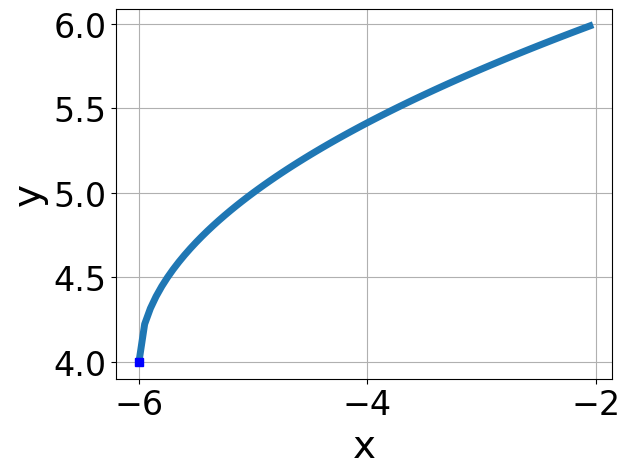
\includegraphics[width=0.5\textwidth]{../Figures/radicalGraphToEquationB.png}
\end{center}
\begin{enumerate}[label=\Alph*.]
\item \( f(x) = - \sqrt[3]{x + 6} - 6 \)
\item \( f(x) = - \sqrt[3]{x - 6} - 6 \)
\item \( f(x) = \sqrt[3]{x - 6} - 6 \)
\item \( f(x) = \sqrt[3]{x + 6} - 6 \)
\item \( \text{None of the above} \)

\end{enumerate} }
\litem{
Choose the graph of the equation below.\[ f(x) = \sqrt[3]{x - 12} + 6 \]\begin{enumerate}[label=\Alph*.]
\begin{multicols}{2}\item 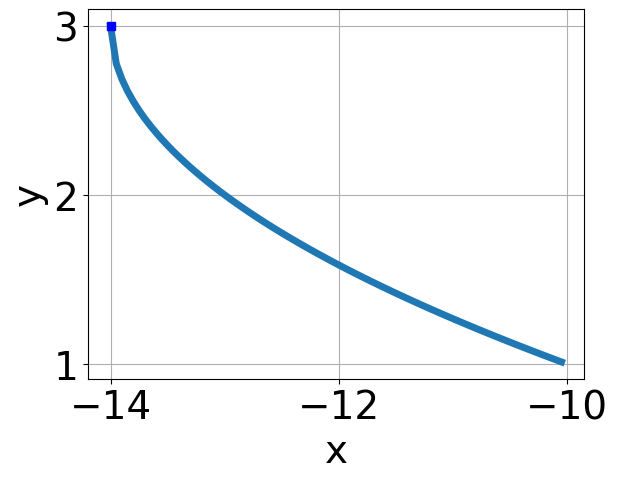
\includegraphics[width = 0.3\textwidth]{../Figures/radicalEquationToGraphCopyAB.png}\item 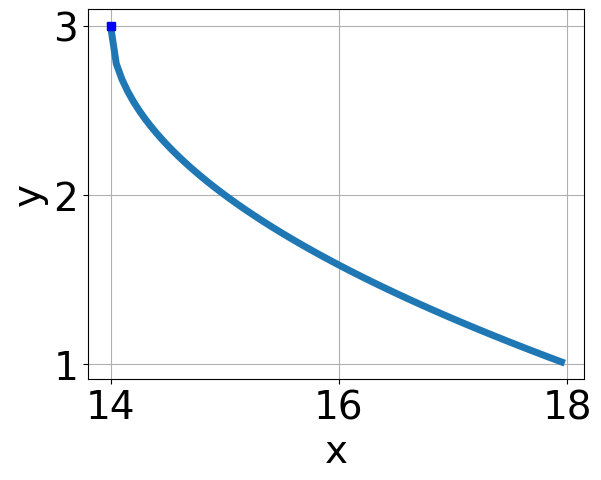
\includegraphics[width = 0.3\textwidth]{../Figures/radicalEquationToGraphCopyBB.png}\item 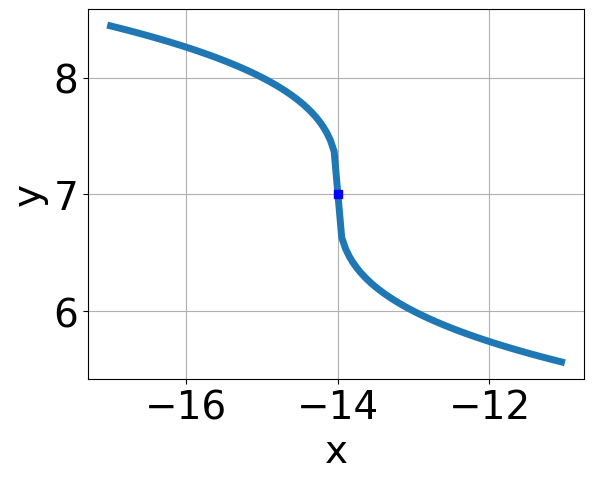
\includegraphics[width = 0.3\textwidth]{../Figures/radicalEquationToGraphCopyCB.png}\item 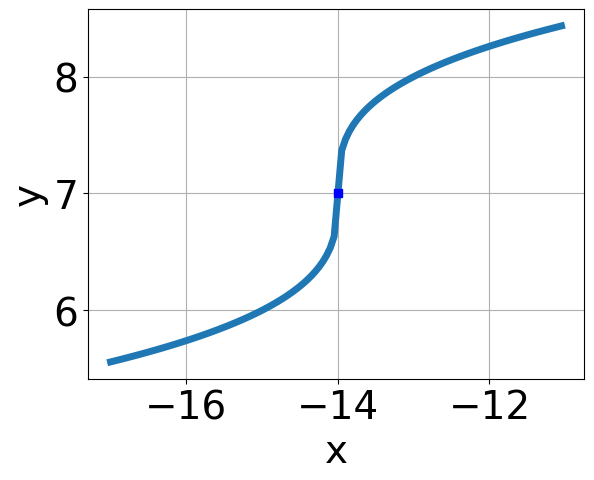
\includegraphics[width = 0.3\textwidth]{../Figures/radicalEquationToGraphCopyDB.png}\end{multicols}\item None of the above.
\end{enumerate} }
\litem{
Choose the graph of the equation below.\[ f(x) = \sqrt[3]{x - 6} + 5 \]\begin{enumerate}[label=\Alph*.]
\begin{multicols}{2}\item 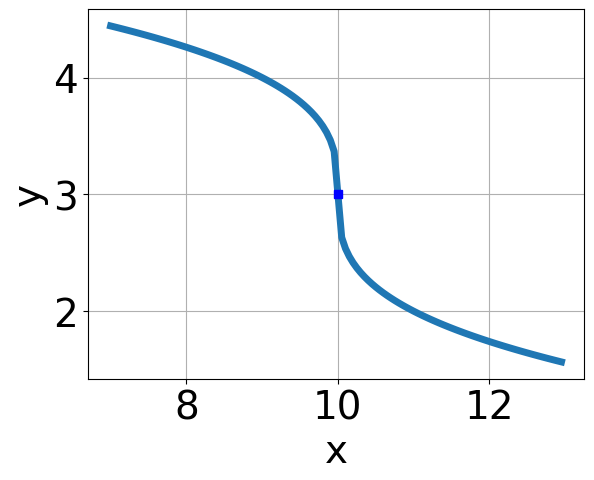
\includegraphics[width = 0.3\textwidth]{../Figures/radicalEquationToGraphAB.png}\item 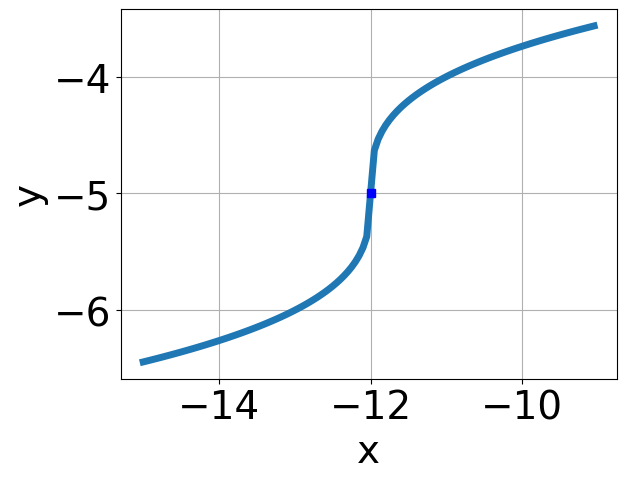
\includegraphics[width = 0.3\textwidth]{../Figures/radicalEquationToGraphBB.png}\item 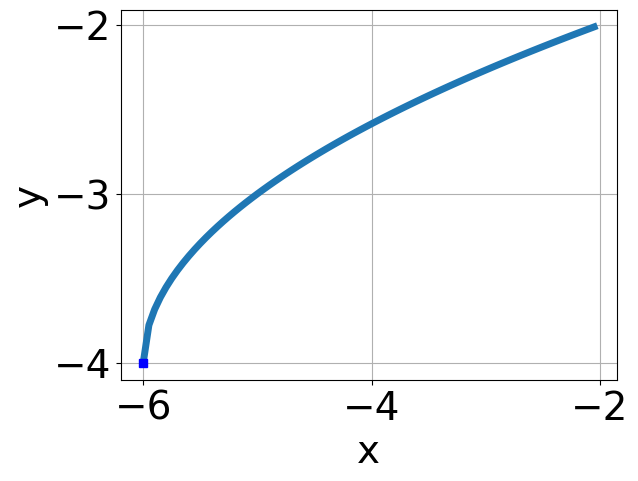
\includegraphics[width = 0.3\textwidth]{../Figures/radicalEquationToGraphCB.png}\item 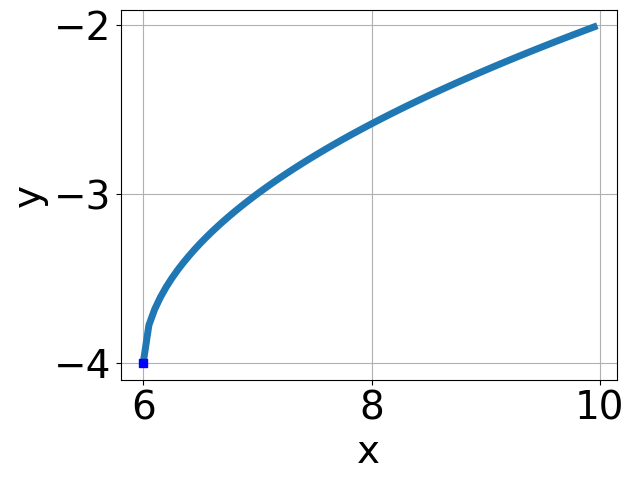
\includegraphics[width = 0.3\textwidth]{../Figures/radicalEquationToGraphDB.png}\end{multicols}\item None of the above.
\end{enumerate} }
\litem{
What is the domain of the function below?\[ f(x) = \sqrt[4]{-8 x - 5} \]\begin{enumerate}[label=\Alph*.]
\item \( (-\infty, a], \text{where } a \in [-3.8, -1.2] \)
\item \( (-\infty, \infty) \)
\item \( [a, \infty), \text{where } a \in [-1.07, -0.3] \)
\item \( [a, \infty), \text{where } a \in [-2.42, -1.37] \)
\item \( (-\infty, a], \text{ where } a \in [-1.1, -0.4] \)

\end{enumerate} }
\litem{
Choose the equation of the function graphed below.
\begin{center}
    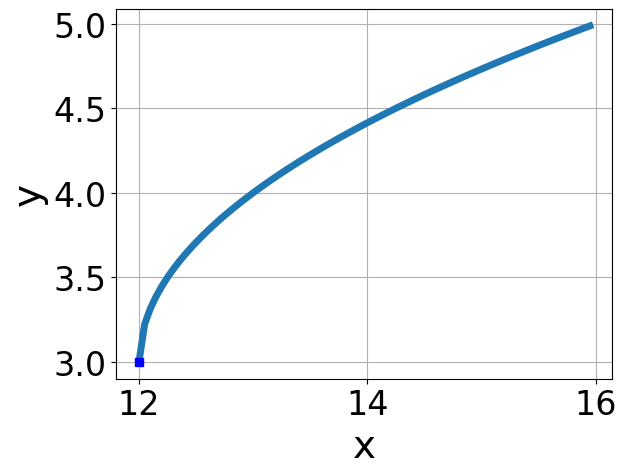
\includegraphics[width=0.5\textwidth]{../Figures/radicalGraphToEquationCopyB.png}
\end{center}
\begin{enumerate}[label=\Alph*.]
\item \( f(x) = - \sqrt[3]{x - 12} + 3 \)
\item \( f(x) = \sqrt[3]{x + 12} + 3 \)
\item \( f(x) = - \sqrt[3]{x + 12} + 3 \)
\item \( f(x) = \sqrt[3]{x - 12} + 3 \)
\item \( \text{None of the above} \)

\end{enumerate} }
\litem{
Solve the radical equation below. Then, choose the interval(s) that the solution(s) belongs to.\[ \sqrt{-14 x^2 - 54} - \sqrt{-75 x} = 0 \]\begin{enumerate}[label=\Alph*.]
\item \( x_1 \in [-2.1, -0.1] \text{ and } x_2 \in [-7.5,-2.5] \)
\item \( x_1 \in [-0.5, 1.9] \text{ and } x_2 \in [3.5,7.5] \)
\item \( x \in [-0.5,1.9] \)
\item \( \text{All solutions lead to invalid or complex values in the equation.} \)
\item \( x \in [1.8,8.8] \)

\end{enumerate} }
\litem{
What is the domain of the function below?\[ f(x) = \sqrt[3]{-5 x - 7} \]\begin{enumerate}[label=\Alph*.]
\item \( \text{The domain is } [a, \infty), \text{   where } a \in [-1.05, -0.1] \)
\item \( \text{The domain is } [a, \infty), \text{   where } a \in [-2.22, -1] \)
\item \( \text{The domain is } (-\infty, a], \text{   where } a \in [-1.33, 1.27] \)
\item \( (-\infty, \infty) \)
\item \( \text{The domain is } (-\infty, a], \text{   where } a \in [-1.43, -1.06] \)

\end{enumerate} }
\litem{
Solve the radical equation below. Then, choose the interval(s) that the solution(s) belongs to.\[ \sqrt{-6 x - 7} - \sqrt{-4 x + 7} = 0 \]\begin{enumerate}[label=\Alph*.]
\item \( x_1 \in [-7, -5] \text{ and } x_2 \in [-6.17,-0.17] \)
\item \( \text{All solutions lead to invalid or complex values in the equation.} \)
\item \( x_1 \in [-1.17, -0.17] \text{ and } x_2 \in [-0.25,6.75] \)
\item \( x \in [-7,-5] \)
\item \( x \in [-0,5] \)

\end{enumerate} }
\litem{
Solve the radical equation below. Then, choose the interval(s) that the solution(s) belongs to.\[ \sqrt{-5 x - 4} - \sqrt{6 x - 4} = 0 \]\begin{enumerate}[label=\Alph*.]
\item \( x_1 \in [-0.91, -0.73] \text{ and } x_2 \in [0.32,1.53] \)
\item \( x \in [-0.78,-0.65] \)
\item \( x \in [-0.03,0.05] \)
\item \( \text{All solutions lead to invalid or complex values in the equation.} \)
\item \( x_1 \in [-0.91, -0.73] \text{ and } x_2 \in [-0.28,0.2] \)

\end{enumerate} }
\litem{
Solve the radical equation below. Then, choose the interval(s) that the solution(s) belongs to.\[ \sqrt{54 x^2 - 28} - \sqrt{-39 x} = 0 \]\begin{enumerate}[label=\Alph*.]
\item \( x \in [-6.17,-0.17] \)
\item \( x_1 \in [0.44, 1.44] \text{ and } x_2 \in [0.84,1.26] \)
\item \( x \in [0.44,1.44] \)
\item \( \text{All solutions lead to invalid or complex values in the equation.} \)
\item \( x_1 \in [-6.17, -0.17] \text{ and } x_2 \in [0.1,0.54] \)

\end{enumerate} }
\end{enumerate}

\end{document}